\clearpage
\section{Směšovací blok}
\indent\indent Tento obvod má za úkol frekvenčně posunout přijímaný napěťový signál do základního nízkofrekvenčního (audio) pásma, tak aby jej bylo možné zpracovávat pomocí zvukové karty. Výstupem s tohoto modulu jsou dva signály I a Q navzájem posunuty o $\frac{\pi}{2}$. Signály I a Q jsou přiváděny na linkový vstup zvukové karty.

\subsection{Popis funkce bloku}
\indent\indent Do obvodu vstupují dva napěťové signály, jeden s lokálního oscilátoru a druhý ze selektivního zesilovače. Signál ze selektivního zesilovače jde přes rekonstrukční filtr s mezní frekvencí $35~MHz$, který odstraňuje vysokofrekvenční šum a vyšší harmonické frekvence, které nepotlačil první rekonstrukční filtr po digitální syntéze.

% rekonstrukční filtr
\begin{figure}[H]
	\centering
	\includegraphics[width=170mm]{img/mix/filtr.pdf}
	\caption{Graf napěťového přenosu rekonstrukčního filtru}    		
\end{figure}

Signál je přiveden do diodového kruhového směšovače, ten ale potřebuje, aby vstupní signál měl úroveň nejméně $7~dBm$. Proto je zesílen v třístupňovém zesilovači, tvořeném kaskádově řazenými zesilovači, pracujícími ve třídě A. Nejprve se signál zesiluje napěťově v prvních dvou stupních postavených s tranzistory KF190, poté je signál výkonově zesílen v zesilovači založeném opět na tranzistoru KF630D. Tento zesilovač je opět obdobný, jako vstupní zesilovač popsaný ve druhé kapitole, s tím rozdílem, že transformátor je tentokrát navinutý na toroidním jádru s materiálu N5. Po zesílení je signál přiveden do již zmíněného diodového kruhového směšovače, založeném na rychlých Schottkyho diodách KAS44 a transformátorech T4 a T5. KAS44 je diodový směšovač. Uvnitř KAS44 se nacházejí čtyři vyvážené diody. Po smíšení je signál přiveden na paralelní pásmovou propust, skládající se ze dvou rezonančních obvodů. První rezonanční obvod se skládá z kondenzátorů C17, C18 a T2 a je naladěn na $5,7~MHz$. Druhý rezonanční obvod se skládá z kondenzátorů C12, C13 a transformátoru T1. Tento obvod rezonuje na kmitočtu $6,0~MHz$. Paralelní obvody spojuje dohromady vazební kondenzátor C16. Za touto pásmovou propustí je tedy mezifrekvenční signál o kmitočtu $5,7-6,0~MHz$. Tento mezifrekvenční signál je dále zpracováván. Křemíkový oscilátor XTAL1 rezonuje na frekvenci $24,0~MHz$ a vytváří sinusové napětí. Sinusové napětí z křemíkového oscilátoru je opět vytvarováno tvarovačem impulzů tvořeným integrovaným obvodem IC1. Poté upravený hodinový signál pokračuje do integrovaného obvodu U1. U1 je obvod 74F74, který má v sobě integrované dva klopné obvody typu D. U1 je zapojen jako 2b Johnsův čítač, to znamená, že na výstupu generuje dva signály navzájem posunuté o $\frac{\pi}{2}$. Během čtyř taktů oscilátoru se na výstupu Johnsova čítače prostřídají všechny možné stavy. Výstup Johnsova čítače je použit jako adresový vstup pro obvod U3. U3 je digitálně řízený přepínač založený na technologii MOS-FET. U3 postupně přepíná své 4 polohy. Na vstupu přepínače je přiveden mezifrekvenční signál. Na spínače obvodu U3 jsou připojeny kondenzátory C22, C25, C26 a C28. Slouží zde jako analogová paměť. Každý kondenzátor je jednou za periodu  mezifrekvence sepnut a nabíjen. Přepínání poloh spínačů a následné nabíjení kondenzátorů jsou posunuty v čase o $\frac{\pi}{2}$. Tím, že jsou kondenzátory spínány dochází ke směšování. Jedná se o podobnou myšlenku jako při spínání diody, s tím rozdílem, že kondenzátor  je nabíjen a pak se po zbytek času vybíjí. Na kondenzátorech jsou tedy čtyři napěťové průběhy posunuté o $\frac{\pi}{2}$ v nízko frekvenčním pásmu. Proto se tomuto zapojení říká kvadraturní detektor. (Podle svého objevitele někdy též nazývaný Tayloe detector). Vzhledem k tomu že na výstupu jsou signály posunuty o $\frac{\pi}{2}$, tak je zjevné, že dva z nich nesou redundantní informaci. Tedy na kondenzátoru C22 je napěťový průběh posunut o $\frac{\pi}{2}\pi$. Na kondenzátoru C25 je ten samý průběh ale posunutý o $\frac{3\pi}{2}$. Tedy v podstatě invertovaný průběh co je na kondenzátoru C22. Proto jsou tato dvě napětí přivedeny do diferenciálního zesilovače postaveném na operačním zesilovači U4. U4 je špičkový operační zesilovač AD8055 s nízkým zkreslením a šumem, pracující až do frekvence $300~MHz$. Díky tomu, že jsme sečetli redundantní signál se signálem který jsme potřebovali, tak jsme dostali na výstupu zesílený signál. Obdobně se zpracují zbylé dva signály po kvadraturním směšování z kondenzátorů C26 a C28. Na těchto kondenzátorech jsou napěťové průběhy posunuty o $0\pi$ a $\pi$. Za diferenciálními zesilovači jdou tantalové kondenzátory C34 a C35, které slouží k oddělení stejnosměrné složky od střídavých napěťových signálů a snižují  offset při následné digitalizaci signálu ve zvukové kartě. Za kondenzátory C34 a C35 jsou tedy již signály I a Q, které slouží k softwarové demodulaci.

% schéma
\begin{landscape}
	\begin{figure}[h]
		\centering 	
		\includegraphics[height=\textwidth]{img/mix/sch.pdf}
		\caption{Schéma zapojení směšovacího bloku}	
	\end{figure}
\end{landscape}
%\includepdf[landscape=true]{img/mix/sch.pdf}

% DPS
\begin{figure}[H]
	\centering
	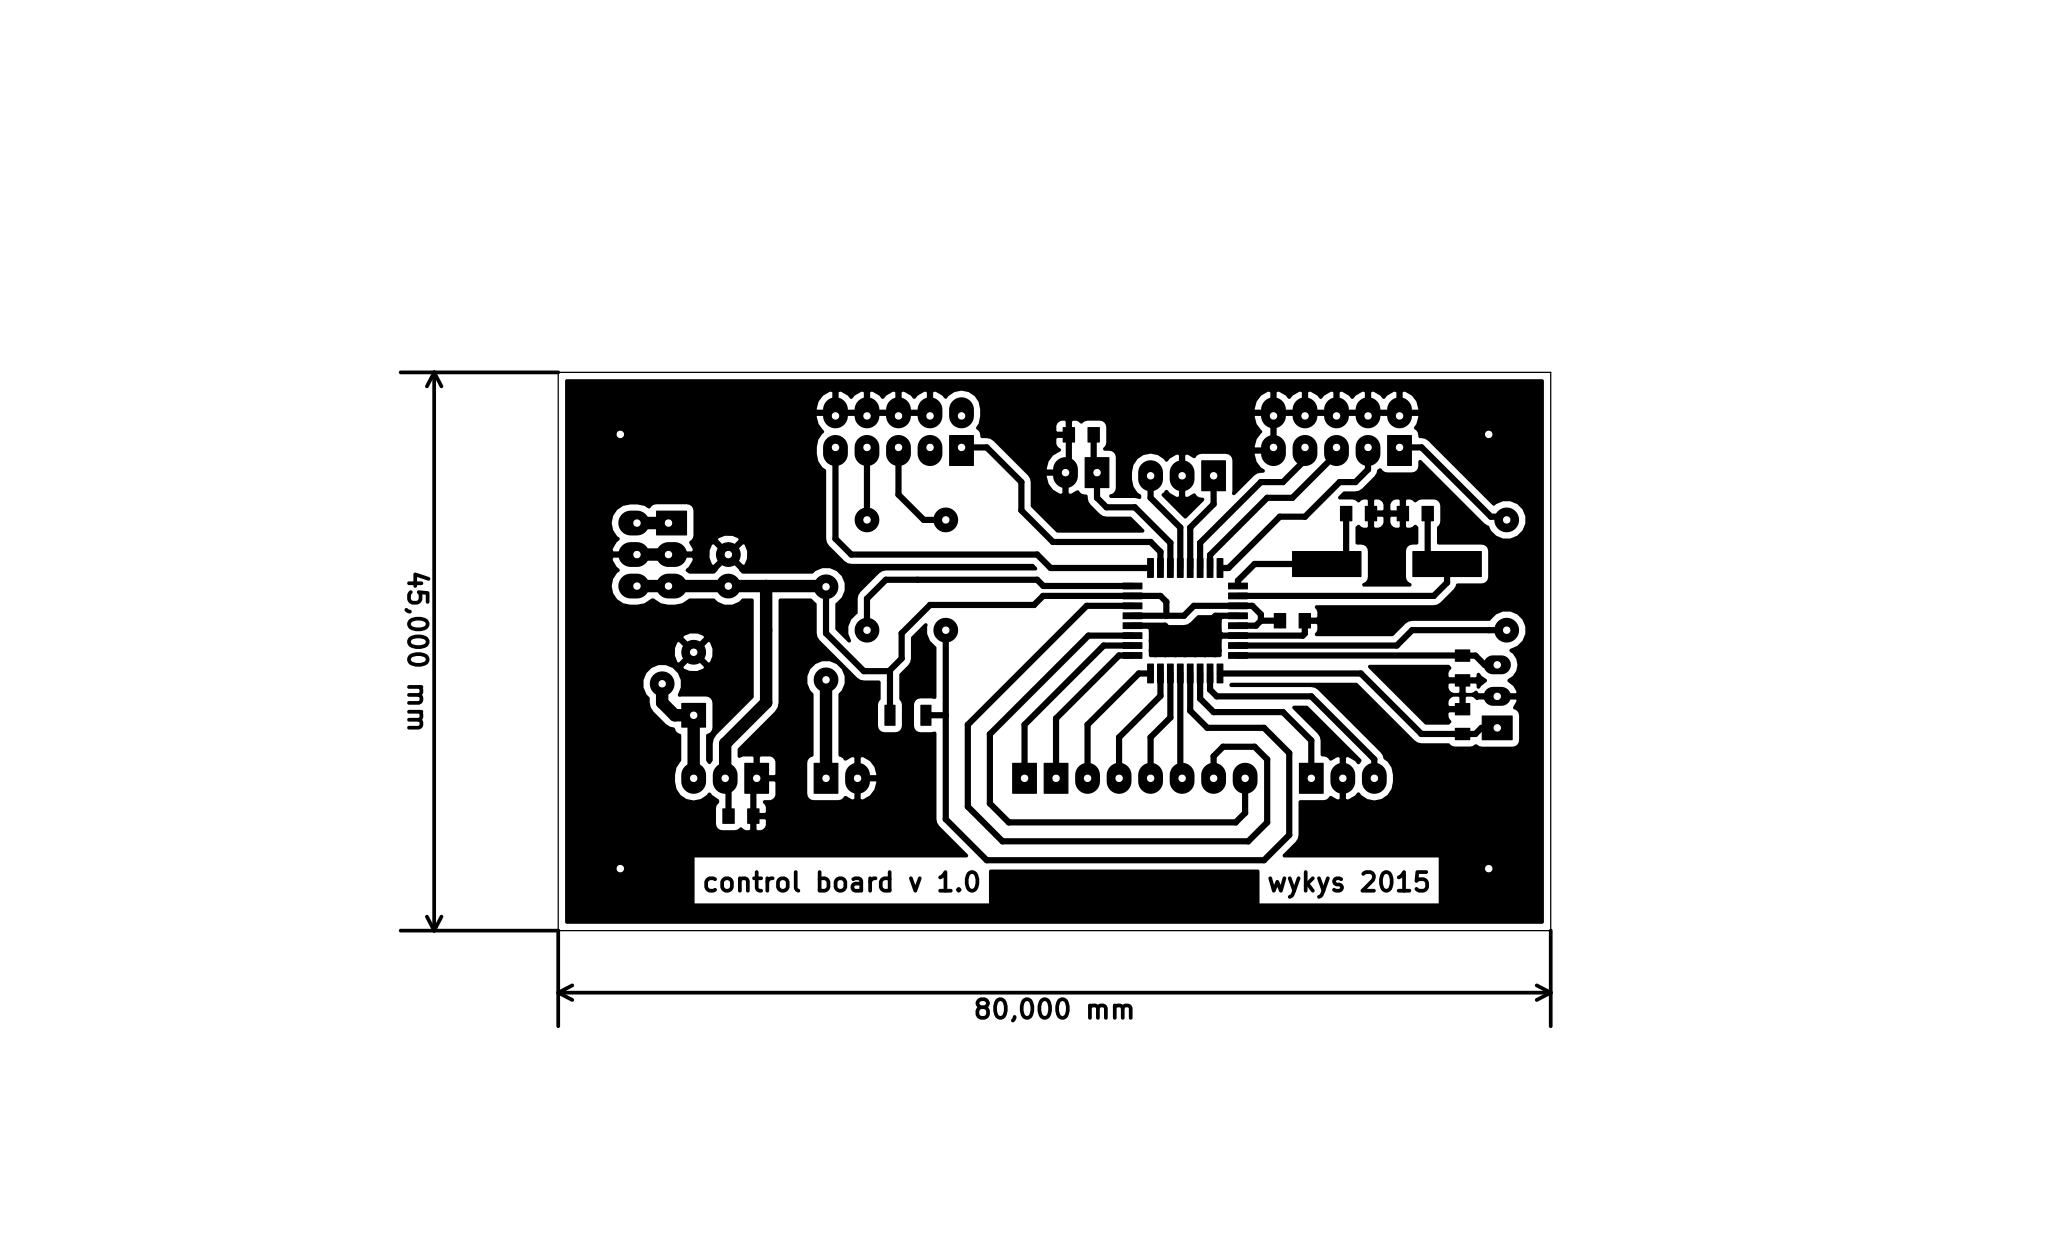
\includegraphics[width=170mm]{img/mix/cu_b.pdf}
	\caption{Deska plošného spoje směšovacího bloku, strana spojů}    		
\end{figure}

% os f
\begin{figure}[H]
	\centering
	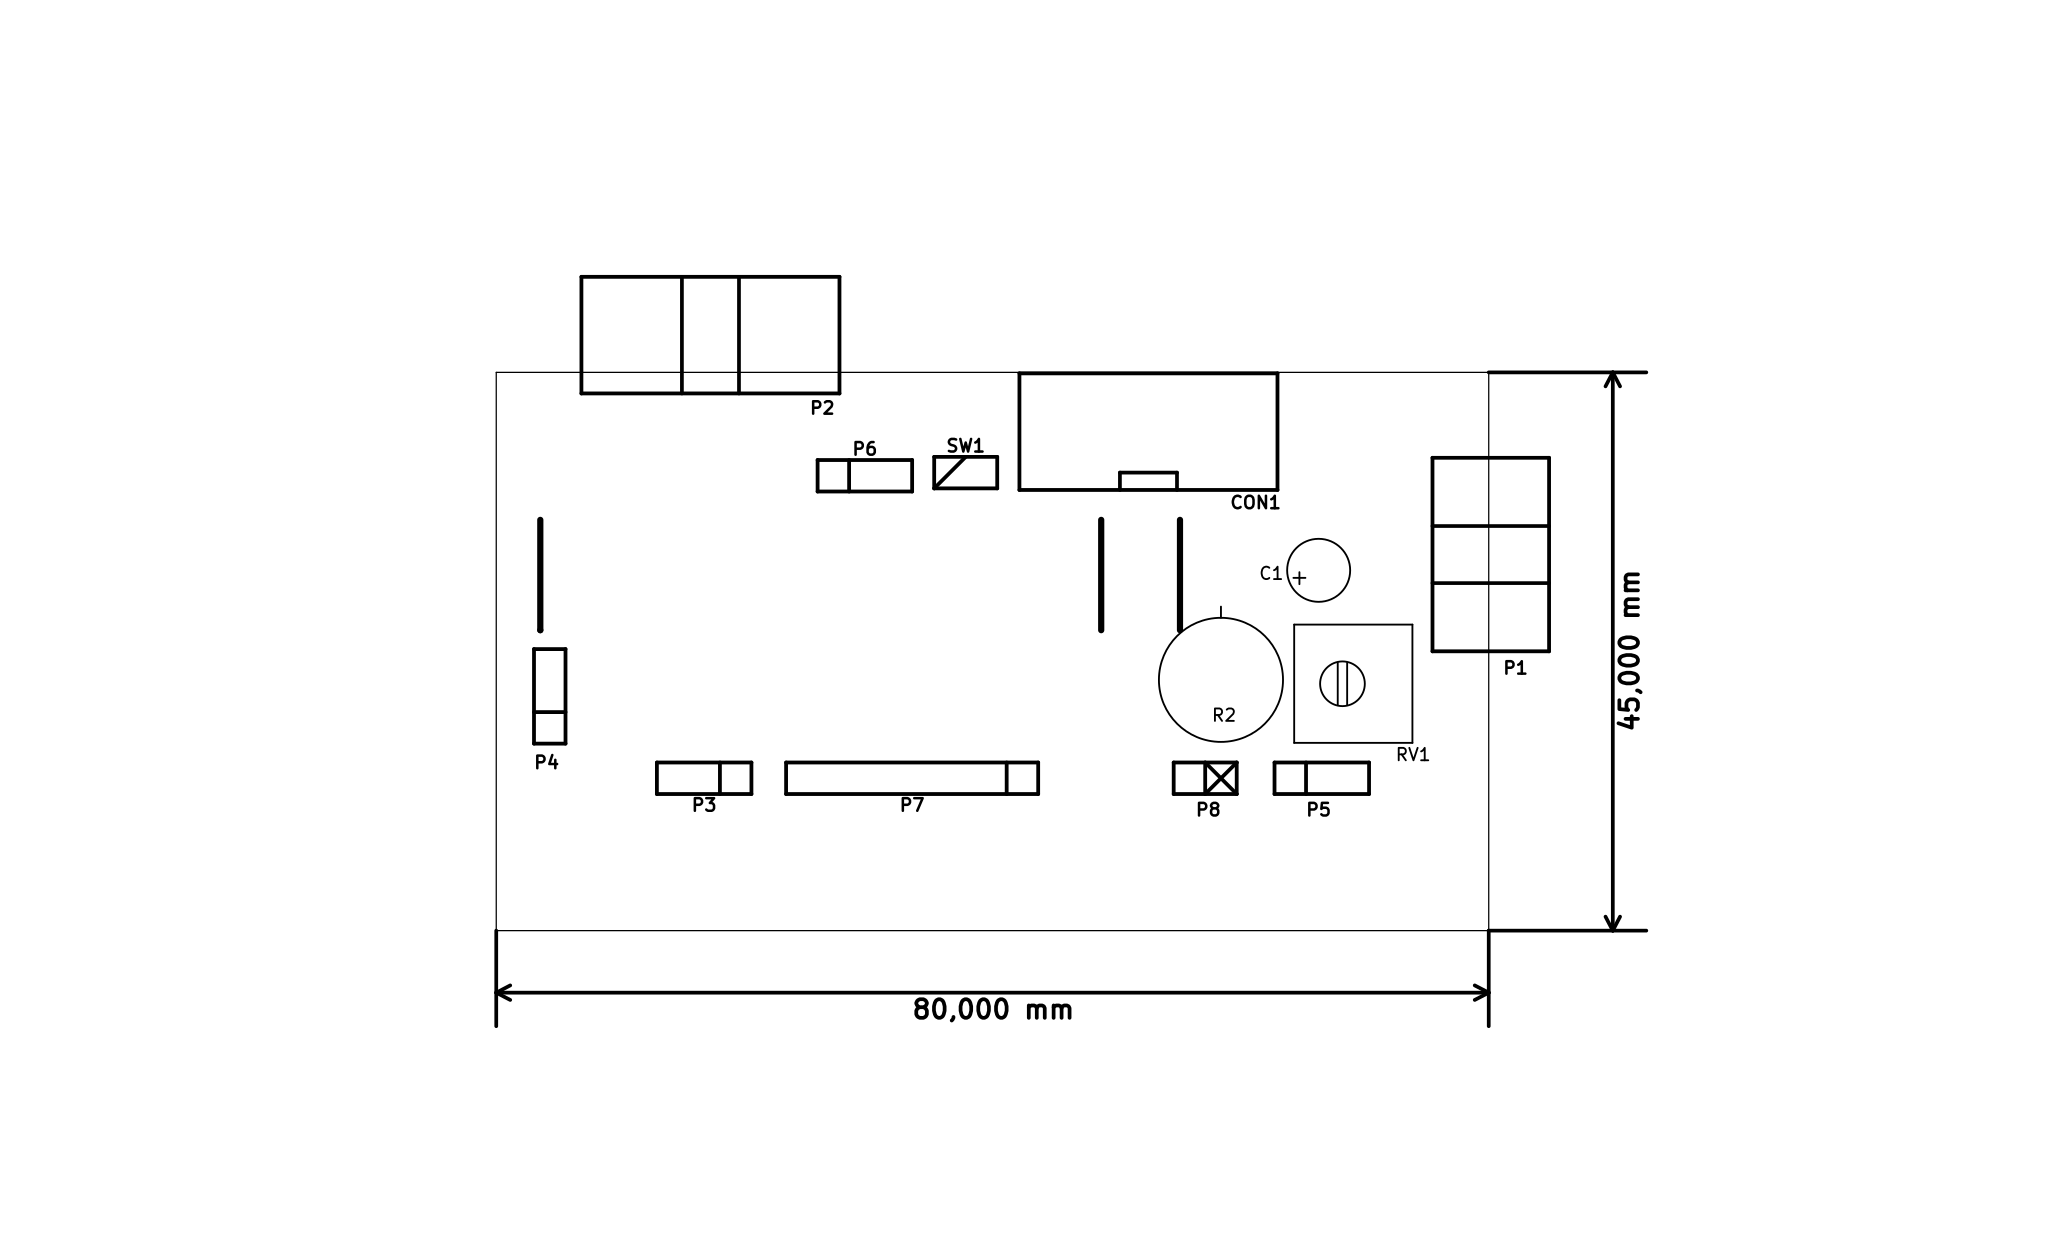
\includegraphics[width=170mm]{img/mix/os_f.pdf}
	\caption{Osazovací plán směšovacího bloku, strana součástek}    		
\end{figure}

% os b
\begin{figure}[H]
	\centering
	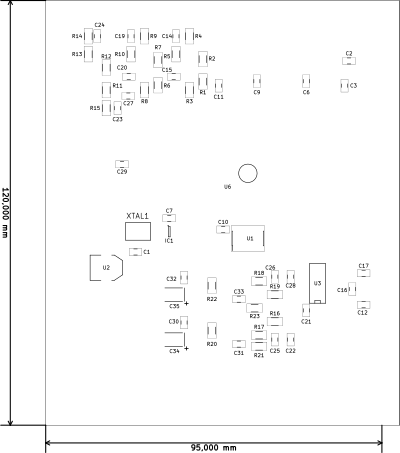
\includegraphics[width=170mm]{img/mix/os_b.pdf}
	\caption{Osazovací plán směšovacího bloku, strana spojů}    		
\end{figure}

\begin{table}[H]
	\begin{center}
		\caption{Tabulka použitých součástek pro desku DDS}
		\label{tab:mix_os}    
		\begin{tabular}[H]{!{\vrule width 1pt}c|c|c|c!{\vrule width 1pt}}
		    \specialrule{1pt}{0pt}{0pt} 
		    \textbf{Určovatel}	&	\textbf{Pouzdro}	&	\textbf{Množství}	&	\textbf{Určení}	\\\specialrule{1pt}{0pt}{0pt} 			
			M1,M2,M3,M4	&	M3	&	5	&	M3	\\\hline
			T1,T2	&	Amidon-T-44-2	&	2	&	TRXTOY	\\\hline
			T5,T4	&	Inductor\_choke	&	2	&	TRMIX	\\\hline
			T3	&	N5	&	1	&	TR11	\\\hline
			C1,C2,C7,C10	&	C\_0805	&	4	&	100n	\\\hline
			C14,C15,C19-C33	&	C\_0805	&	17	&	100n	\\\hline
			C3,C11	&	C\_0805	&	2	&	47p	\\\hline
			C4,C5	&	Elko\_vert\_11x5mm\_RM2.5	&	2	&	100u/35V	\\\hline
			C6,C9	&	C\_0805	&	2	&	180p	\\\hline
			C8	&	Elko\_vert\_11x5mm\_RM2.5	&	1	&	22u/10V	\\\hline
			C12,C17	&	C\_0805	&	2	&	150p	\\\hline
			C13,C18	&	CT	&	2	&	6-50p	\\\hline
			C16	&	C\_0805	&	1	&	4p7	\\\hline
			C34,C35	&	Tantal\_Size\_B	&	2	&	10u/10V	\\\hline
			IC1	&	SOT-23-5	&	1	&	74VHC1G132DTT1G	\\\hline
			L1,L3	&	Amidon-T44-2	&	2	&	300n	\\\hline
			L2	&	Amidon-T-44-2	&	1	&	480n	\\\hline
			P1	&	MCX	&	1	&	LO	\\\hline
			P2,P3	&	vasch\_strip\_3x2\_90	&	2	&	MLW6	\\\hline
			P4	&	Socket\_Strip\_Straight\_1x03	&	1	&	PSH02-3WG	\\\hline
			P5	&	MCX	&	1	&	RF	\\\hline
			Q3	&	TO5	&	1	&	KF630D	\\\hline
			R1,R6	&	R\_1206	&	2	&	6k8	\\\hline
			R2,R7	&	R\_1206	&	2	&	1k2	\\\hline
			R3,R8	&	R\_1206	&	2	&	390R	\\\hline
			R4,R9	&	R\_1206	&	2	&	68R	\\\hline
			R5,R10	&	R\_1206	&	2	&	150R	\\\hline
			R11	&	R\_1206	&	1	&	560R	\\\hline
			R12	&	R\_1206	&	1	&	500R	\\\hline
			R13	&	R\_1206	&	1	&	4R7	\\\hline
			R14	&	R\_1206	&	1	&	12R	\\\hline
			R15	&	R\_1206	&	1	&	3k3	\\\hline
			R16,R17,R18,R19	&	R\_1206	&	4	&	1k	\\\hline
			R20,R21,R22,R23	&	R\_1206	&	4	&	10k	\\\hline
			U1	&	SOIC-14	&	1	&	74F74	\\\hline
			U2	&	SOT-223	&	1	&	LD1117S33CTR	\\\hline
			U3	&	SO-16-N	&	1	&	74HC4051	\\\hline
			U4,U5	&	DIP-8	&	2	&	AD8055	\\\hline
			U6	&	M234\_NoHole\_Housing	&	1	&	KAS44	\\\hline
			XTAL1	&	SMD7x5	&	1	&	CFPS	\\\hline
			Q2,Q1	&	TO-92\_Rugged\_Reverse	&	2	&	KF190 \\\specialrule{1pt}{0pt}{0pt} 
		\end{tabular}  
	\end{center}
\end{table}

